\documentclass[11pt]{beamer}
\usetheme{CambridgeUS}
\usecolortheme{orchid}

\usepackage[utf8]{inputenc}
\usepackage[brazil]{babel}
\usepackage[T1]{fontenc}

\usepackage{amsmath}
\usepackage{amsfonts}
\usepackage{amssymb}
\usepackage{graphicx}
\usepackage{setspace}
\usepackage{ragged2e}


\setbeamertemplate{caption}[numbered]
\setbeamercovered{transparent} 
\setbeamertemplate{navigation symbols}{}

\author[Joao Victor]{% 
	Joao Victor\inst{1}}
\title[Moodle]{Modular Object-Oriented Dynamic Learning Environment}
\institute[]{% 	
	\textsuperscript{1} Graduando em Matemática
}
\titlegraphic{
\includegraphics[width=0.2\textwidth]{imagens/logo_3.jpg}}
\date{\today} 
%\subject{}

% ---------------------------------------------------------

\begin{document}
\justifying
\onehalfspacing 

\begin{frame}
    \titlepage
\end{frame}

\begin{frame}{Sumário}
	\tableofcontents
\end{frame}

\section{Introdução}

	\begin{frame}{Introdução}
		
		\begin{itemize}
			\justifying
			\item O contexto educacional vem sofrendo inúmeras transformações e mudanças, e assim, o ensino a distância vem ganhando espaço, porém alunos e professores precisam assumir novos papéis.
			
			\uncover<2->{
			\item Assim, com o avanço da tecnologia e o crescimento do ensino a distância fez-se necessário o surgimento de ambientes de aprendizagem inteligentes e dinâmicos que permitissem oferecer um ensino mais democrático, para todos. (Lima, 2021) 
			}
			
			\uncover<3->{
			\item Vamos conhecer, então, sobre o Moodle, que é uma das plataformas de aprendizagem mais utilizadas atualmente, no planeta, seus benefícios e características.
			}
		\end{itemize}
	\end{frame}

\section{A origem do Moodle}

	\begin{frame}{A origem do Moodle}
		\begin{block}{A origem do Moodle}
			\begin{itemize}
				\justifying
				\item Em 1970, Martin Dougiamas, o criador do Moodle, estudava no deserto da Austrália, por meio do rádio e de material que lhe era enviado por correspondência (uma das formas inovadoras originais do ensino a distância). Era o início de seu interesse pelo ensino a distância.
				
				\item Em 1999, enquanto estudava na Curtin University, começou a idealizar o Moodle como pesquisa para a obtenção de seu título de Phd. Em 2002, ocorreu o lançamento da versão 1.0 do Moodle, já como um software livre e gratuito. 
			\end{itemize}
		\end{block}
	\end{frame}
	
	\begin{frame}{A origem do Moodle}
		\begin{block}{A origem do Moodle}
			\begin{itemize}
				\justifying
				\item Em pouquíssimo tempo, o mundo já usava e se encantava pela plataforma. Em 2008, seu criador recebeu o prêmio ‘Open Source' na categoria Enabler na educação, por causa do Moodle.
				
				\item E em 2005, tornou-se o AVA mais popular do mundo, alcançando cerca de 223 países e um enorme número de usuários (Lima, 2021). Em 2022, o Moodle completou 20 anos.
			\end{itemize}
		\end{block}
	\end{frame}
	
	\begin{frame}{A origem do Moodle}
		Os 8 países que mais usam o Moodle (Lima, 2021)
		
		$$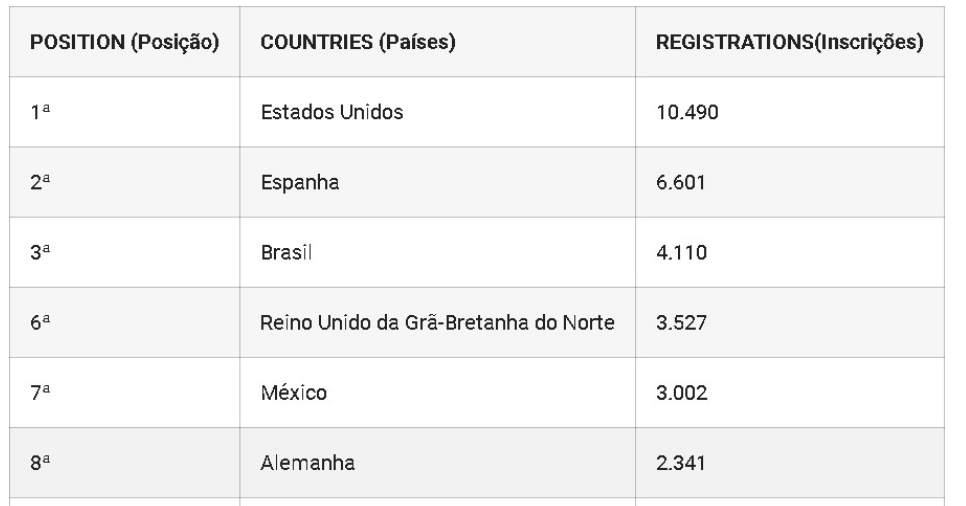
\includegraphics[scale=0.3]{imagens/ranking.png}$$
	\end{frame}

\section{O Moodle}
	\begin{frame}{O Moodle}
		\begin{itemize}
			\justifying
			\item Em inglês, a sigla representa o \textit{Modular Object-Oriented Dynamic Learning Environment};
			\item Em português, Ambiente de Aprendizado Modular Orientado ao Objeto;
			\item É uma plataforma digital, um software livre, desenvolvido para a produção de cursos e de sites na internet;
			\item Pode ser configurado conforme as características dos cursos e suas necessidades.
		\end{itemize}
	\end{frame}
	
	\begin{frame}{O Moodle}
		\justifying É uma plataforma amigável, intuitiva e com acesso facilitado, que apresenta uma série de recursos que auxiliam no ensino, sendo possível:
		
		\begin{itemize}
			\justifying
			\item inserir e disponibilizar materiais didáticos;
			\item realizar diversos tipos de atividades e avaliações;
			\item propor debates e conversas;
			\item interagir;
			\item obter informações, etc. (Criativa EaD, 2020)
		\end{itemize}
	\end{frame}
	
	\begin{frame}{O Moodle}

		\begin{itemize}
			\justifying
			\item Funciona como uma sala de aula on-line na qual os docentes podem compartilhar os materiais com os conteúdos das disciplinas, propor atividades e estimular debates por meio dos fóruns.
			\item Os estudantes, por sua vez, podem interagir, baixar os materiais para estudo, obtendo diversas trocas de conhecimento e arquivos multimídia.
		\end{itemize}
	\end{frame}
	
\section{As características do Moodle}

	\begin{frame}{As características do Moodle}
		\begin{block}{As características do Moodle}
			\begin{itemize}
				\justifying
				\item Um dos grandes objetivos da plataforma Moodle é propiciar uma pedagogia socioconstrutivista, 100\% on-line, por meio da colaboração, da reflexão crítica, de discussões e interações que permitam a troca contínua de conhecimentos. 
				
				\item O Moodle tem uma interface simples, eficiente, leve e fácil de instalar, e também é seguro porque seus formulários são checados, os cookies são decodificados e os dados são validados.
			\end{itemize}
		\end{block}
	\end{frame}
	
	\begin{frame}{As características do Moodle}
		\justifying Dentre suas características, podemos citar:
		
		\begin{itemize}
			\justifying
			\item \textbf{uso gratuito:}  seu uso é livre e grátis;
			\item \textbf{flexibilidade:}  várias funcionalidades podem ser inseridas conforme as necessidades das instituições; 
			\item \textbf{adaptabilidade:}  é possível sua adaptação para qualquer negócio;
			\item \textbf{apresenta atualizações:}  acompanhadas por um comunidade desenvolvedora;
			\item \textbf{possui funcionalidade modular: }  apresenta módulos plug-ins que podem ser inseridos no software conforme as necessidades;
			\item \textbf{não é estático:}  recursos novos podem ser adaptados.
		\end{itemize}
	\end{frame}
	
	\begin{frame}{As características do Moodle}
		\begin{itemize}
			\justifying
			\item Além dessas características, o Moodle possui ainda recursos de gamificação que deixam os cursos mais dinâmicos e lúdicos. Os emblemas existentes dentro da plataforma, como as medalhas, vão sendo entregues ao estudante conforme ele vai concluindo as atividades solicitadas.
			
			\uncover<2->{
			\item Uma outra caraterística muito importante, se não for a mais importante, é a \textbf{aprendizagem colaborativa}, visto que os estudantes conseguem expor seus pontos de vista por meio de suas participações síncronas e assíncronas em chats e fóruns, interagindo com os colegas e mediadores, participando ativamente de seu processo de aprendizagem. (Lima, 2021)}
		\end{itemize}
	\end{frame}

\section{As principais ferramentas e recursos}
	\begin{frame}{As principais ferramentas e recursos}
		\begin{itemize}
			\justifying
			\item Por meio das suas ferramentas, eles têm acesso aos materiais, elaboram textos, participam de debates e reflexões, fazem atividades e testes, desenvolvem pesquisas, reveem os resultados das atividades, verificam seu desempenho, entre outras funções.
			\uncover<2->{
			\item Dentre os módulos, encontramos o módulo tarefa, o módulo chat, o módulo pesquisa de opinião, o módulo fórum, o módulo questionário, o módulo recursos, o módulo pesquisa e avaliação e o módulo laboratório de avaliação.}
			
			\uncover<3->{
			\item Os questionários, por exemplo, podem ser utilizados para autoavaliação, lista de exercícios, testes rápidos, provas virtuais, etc. (Prado \& Freitas, 2015)}
		\end{itemize}
	\end{frame}
	
	\begin{frame}{As principais ferramentas e recursos}
		\justifying Exemplos de atividades do Moodle
		
		$$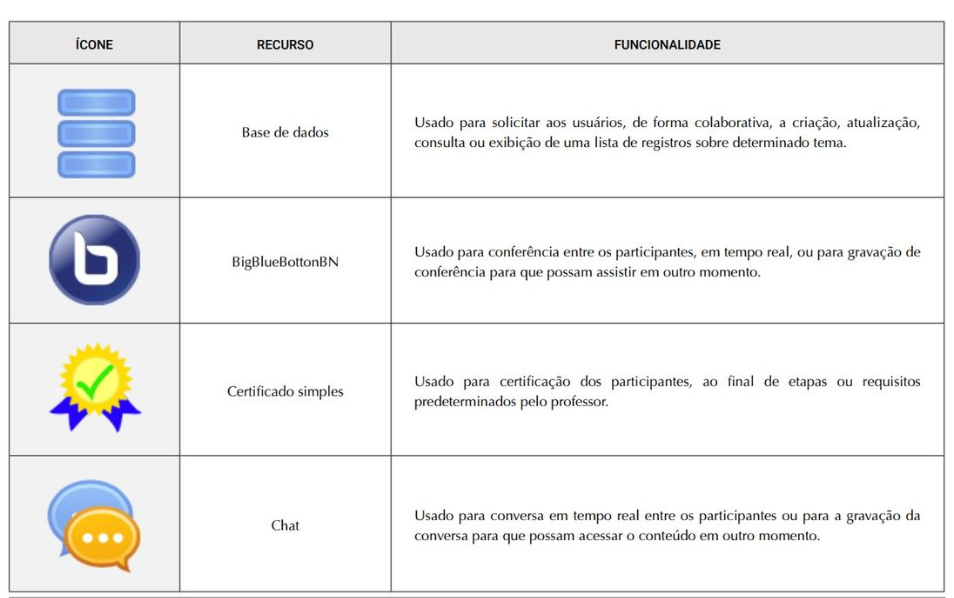
\includegraphics[scale=0.29]{imagens/atividades_moodle.png}$$
	\end{frame}

\section{Em resumo}
	\begin{frame}{Em resumo}
		\justifying Em resumo:
		\begin{itemize}
			\justifying
			\item O Moodle funciona como uma sala de aula on-line na qual os docentes podem compartilhar os materiais com os conteúdos das disciplinas, propor atividades e estimular debates por meio dos fóruns.
			
			\uncover<2->{
			\item Os estudantes, por sua vez, podem interagir, baixar os materiais para estudo, obtendo diversas trocas de conhecimento e arquivos multimídia.}
			
			\uncover<3->{
			\item A plataforma possui uma série de recursos e utilidades que amplificam a sua importância como um AVA completo e atrativo.}
		
		\end{itemize}
	\end{frame}
	
	\begin{frame}{Em resumo}
		\justifying 
		Por meio das suas ferramentas, os estudantes têm acesso aos materiais, elaboram textos, participam de debates e reflexões, fazem atividades e testes, desenvolvem pesquisas, reveem os resultados das atividades, verificam seu desempenho, entre outras funções.
	
	\end{frame}
	
\section{Referências}
	\begin{frame}{Referências}
		\begin{itemize}
			\item Criativa EaD. (2020). O Que É O Moodle E Quais Suas Principais Características?. Disponível em  \href{https://bit.ly/amvb894hg}{Criativa EaD}
			\item Lima, José Maria Maciel. (2021) Plataforma Moodle: A educação por mediação tecnológica. Revista Científica Multidisciplinar Núcleo do Conhecimento. Ano 06, Ed. 01, Vol. 07, pp. 17-37. Disponível em: \href{https://bit.ly/9mb7b2}{<link>} 
			\item Must University. O Moodle como Plataforma de Ensino a Distância. Disponível em: \href{https://edu612tema19v2pt.webflow.io/}{Must University} 
			\item Moodle UTFPR. Disponível em: \href{https://moodle.utfpr.edu.br/login/index.php}{Moodle UTFPR Curitiba}
		\end{itemize}
	\end{frame}
\end{document}